
\section{Prerequisiti matematici}

\subsection*{Classi di funzioni $f:A\rightarrow B$}
\subsubsection*{Iniettive}
$ f \text{ è iniettiva se } \forall a_1,a_2 \in A: a_1\neq a_2
\Rightarrow f(a_1)\neq f(a_2) $
\subsubsection*{Suriettive}
$ f \text{ è suriettiva se } \forall b\in B \ \ \exists a\in A : f(a)=b $
\subsubsection*{Biettive}
$f$ è biettiva se è sia iniettiva che suriettiva.

\subsection*{Composizione di funzioni}
Date $f:A\rightarrow B$ e $g:B\rightarrow C$, si definisce $f$ composto $g$
come la funzione $g\circ f:A\rightarrow C$ come:
$$ g\circ f(a) = g(f(a)) $$
La composizione non è un operatore commutativo.

\subsection*{Funzioni parziali e totali}
La notazione $f(a)$\textdownarrow \ indica che la funzione è definita su $a$, ovvero
che esiste un valore $b$ del codominio tale che $f(a)=b$.

Al contrario, la notazione $f(a)$\textuparrow \ indica che la funzione \textbf{non} è
definita su $a$.

Una funzione $f:A\rightarrow B$ definita su tutto il suo dominio è detta totale. Se 
invece esistono dei valori del dominio nei quali $f$ non è definita, $f$ è detta 
parziale:
$$ f \text{ è \textbf{totale} se } \forall a\in A \ \ f(a)\text{\textdownarrow} $$
$$ f \text{ è \textbf{parziale} se } \exists a\in A : f(a)\text{\textuparrow} $$

\subsubsection*{Campo di esistenza}
Dalla definizione di funzione parziale si intuisce come l'insieme di tutti i valori
nel quale la funzione $f:A\rightarrow B$ è definita, non sempre coincide con il dominio
$A$. Questo insieme è detto \textbf{campo di esistenza di $f$} e si denota con $Dom_f$:
$$ Dom_f = \{ a\in A: f(a)\text{\textdownarrow} \} \subseteq  A $$

\subsubsection*{Totalizzazione di una funzione parziale}
Presa una funzione $f:A\rightarrow B$ parziale, la si può totalizzare, ovvero rendere
totale, aggiungendo al codominio un valore $\perp$ che rappresenta il caso indefinito:
$$ f:A\rightarrow B \ \underset{\text{totalizzazione}}{\longrightarrow} \ 
f:A\rightarrow B \cup \{\perp\}$$
$$ f(a) = \begin{cases}
f(a) & a\in Dom_f\\
\perp & \text{altrimenti}\\
\end{cases} $$
L'insieme $B \cup \{\perp\}$ viene abbreviato con $B_\perp$.

\subsection*{Prodotto cartesiano}
$$ A\times B = \{(a,b):a\in A \wedge b\in B\} $$
L'operatore $\times$ non gode della proprietà commutativa.
$$ \underbrace{A\times A\times\dots\times A}_{n \text{ volte}} = A^n $$

\subsection*{Insiemi di funzioni}
Tutte le funzioni che vanno da $A$ a $B$ è detto $B^A$:
$$ B^A = \{f:A\rightarrow B\} $$
$$ B^A_\perp = \{f:A\rightarrow B_\perp\} $$

\subsection*{Funzione di valutazione}
Si definisce funzione di valutazione $\omega:B_\perp^A\times A \rightarrow B$ con:
$$ w(f,a) = f(a) $$
\begin{itemize}
    \item Fissando $a$ provo tutte le funzioni su $a$;
    \item Fissando $f$ ottengo il suo grafico.
\end{itemize}

\subsection*{Chiusura di insiemi rispetto ad operazioni}
Dato un insieme $U$, si definisce operazione su $U$ una qualunque funzione
$$ op: \underbrace{U\times\dots\times U}_{\displaystyle k=\text{arietà}}\to U $$

L'insieme $A\subseteq U$ è chiuso rispetto all'operazione $op:U^k\to U$ se:
$$ \forall a_1,\dots,a_k \in A : op(a_1,\dots,a_k)\in A $$

Sia $\Omega=\{op_1,\dots,op_t\}$ un insieme di operazioni su $U$, allora $A\subseteq U$
è chiuso rispetto a $\Omega$ se $A$ è chiuso per ogni $op\in\Omega$.

\subsubsection*{Esempi}
Sia $\Omega=\{+,*\}$:
\begin{itemize}
    \item PARI $\subseteq\N$ è chiuso per $\Omega$? Sì, la somma o la moltiplicazione di
        numeri parì è un numero pari.
    \item DISPARI $\subseteq\N$ è chiuso per $\Omega$? No, un controesempio è 
        $3+7=10\notin\text{DISPARI}$.
\end{itemize}

\subsection*{Chiusura di un insieme}

\begin{minipage}{.4\textwidth}
    Sia $A\subseteq U$ e $op:U^k\to U$. Si vuole trovare {\color{red}il più piccolo}
    sottoinsieme di $U$ che: \vspace{.2cm}
    \begin{enumerate}
        \setlength\itemsep{.5em}
        \item {\color{blue}Contiene $A$}
        \item {\color{blue}È chiuso per $op$}
    \end{enumerate}
\end{minipage}
\begin{minipage}{.55\textwidth}
    \begin{center}
        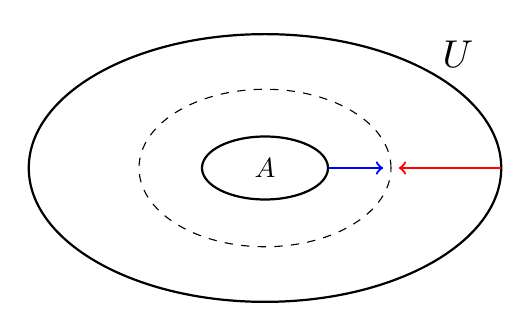
\begin{tikzpicture}
    \node[scale=1.4] at(2.45,1.45) {$U$};
    \draw[thick] (0,0) ellipse (3 and 1.7);
    \draw[dashed] (0,0) ellipse (1.6 and 1);
    \def\x{1.6}
    \draw[->,thick,blue] (.8,0) -- (\x-.1,0);
    \draw[->,thick,red] (3,0) -- (\x+.1,0);
    \draw[thick] (0,0) ellipse (.8 and .4) node {$A$};
\end{tikzpicture}
    \end{center}
\end{minipage}
\vspace{.3cm}

\begin{itemize}
    \item Sicuramente $U$ soddisfa le due condizioni ma {\color{red}si sta cercando
        l'insieme più piccolo};
    \item Se $A$ è chiuso per $op$ allora l'insieme cercato sarebbe $A$ stesso;
    \item Se $A$ non è chiuso per $op$ allora devo {\color{blue} allargare la ricerca ad 
        un insieme più grande}.
\end{itemize}
\vspace{.5em}
\begin{theorem}[Chiusura di un insieme]
    Sia $A\subseteq U$ e $op:U^k\to U$. Il più piccolo sottoinsieme di $U$ contenente $A$
    e chiuso rispetto a $op$ si ottiene calcolando la chiusura di $A$ rispetto a $op$, ovvero
    l'insieme $A^{op}$ definito induttivamente come:
    \begin{enumerate}
        \item $\forall a\in A \ \Rightarrow \ a\in A^{op}$
        \item $\forall a_1,\dots,a_k\in A^{op} \ \Rightarrow \ op(a_1,\dots,a_k)\in A^{op}$
        \item Nient'altro sta in $A^{op}$
    \end{enumerate}
\end{theorem}

Una versione \quotes{più operativa} per trovare $A^{op}$ è:
\begin{enumerate}
    \item $A^{op} = A$
    \item Calcola $op(a_1,\dots,a_k)=r$ su una $k$-tupla di $A$
    \item Se $r\notin A$ allora $A^{op} = A^{op}\cup\{r\}$
    \item Ripeti il punto 2 con un'altra $k$-tupla fino ad averle provate tutte
\end{enumerate}